\chapter{Analiza wymagań i projekt rozwiązania}
Analiza ta pozwala na precyzyjne określenie zadań systemu oraz zaplanowanie jego struktury tak, aby wszystkie komponenty współpracowały bezawaryjnie. Dzięki niej możliwe jest wybranie odpowiednich technologii, które najlepiej sprawdzą się w komunikacji między czujnikiem a aplikacjami końcowymi.

\section{Wymagania funkcjonalne}
Jak pokazano w tabeli \ref{tab:funkcjonalne}, system musi spełniać określone funkcje. Każda z nich została przypisana do odpowiedniego modułu, co ułatwia organizację pracy i pozwala na równoległe rozwijanie poszczególnych części systemu.
\begin{table}[ht!]
\centering
\caption{Wymagania funkcjonalne}
\label{tab:funkcjonalne}
\begin{tabular}{lll}
\toprule
ID & Opis & Priorytet \\  
\midrule
FR-001      & Serwer uruchomiony i działający w oparciu o SpringBoot.    & Wysoki \\
FR-002      & Zapis danych do lokalnej bazy SQL na serwerze.    & Wysoki \\ 
FR-003      & Interfejs użytkownika dostępny przez przeglądarkę i aplikację mobilną.    & Wysoki \\
FR-004      & Wyświetlanie dzinnika zapisów z datą, godziną i wartościami.    & Wysoki \\
FR-005      & Integracja z urządzeniami IoT za pomocą RestAPI.    & Wysoki \\
FR-006      & Implementacja RestAPI do zarządzania danymi i interakcją.    & Wysoki \\
FR-007      & Przygotowanie dokumentacji w oparcu LaTeX. Wymagania edytorskie.    & Wysoki \\
FR-008      & Przygotowanie diagramów UML ilustrujących strukturę i zachowanie systemu.    & Średni \\
FR-009      & Dostarczenie działającej aplikacji.    & Wysoki \\
FR-010      & Utworzenie pliku README.md z opisem projektu i instrukcją instalacji.    & Wysoki \\
FR-011      & Przygotowanie modelu PCB płytki z mikrokontrolerem ESP32 Wroom.    & Średni \\
\bottomrule 
\end{tabular}
\sourcetab{System zasobów - eStudent \parencite{eStudent}}
\end{table}

\section{Wymagania niefunkcjonalne}
Jak pokazano w tabeli \ref{tab:niefunkcjonalne}, system musi spełniać określone standardy wydajności, bezpieczeństwa i kompatybilności.
\begin{table}[ht!]
\centering
\caption{Wymagania niefunkcjonalne}
\label{tab:niefunkcjonalne}
\begin{tabular}{lll}
\toprule
ID & Opis & Priorytet \\  
\midrule
NFR-001      & Czas odpowiedzi API mniejszy niż 300ms.    & Wysoki \\
NFR-002      & Dostępność systemu większa niż 99\%.        & Wysoki \\ 
NFR-003      & Skalowlaność: obsługa min. 1000 jednoczesnych użytkowników.    & Wysoki \\
NFR-004      & Bezpieczeństwo: szyfrowanie SSL/TLS dla transmisji danych.    & Wysoki \\
NFR-005      & Kompatybilność: Android 8.0+, przeglądarki wspierające HTML5.	    & Średni \\
NFR-006      & Dostępność zgodna z WCAG 2.1 na poziomie AA.    & Średni \\
\bottomrule 
\end{tabular}
\sourcetab{System zasobów - eStudent \parencite{eStudent}}
\end{table}

\section{Wymagania jakościowe}
Jak pokazano w tabeli \ref{tab:jeśli_quality}, system musi spełniać określone kryteria jakościowe, aby zapewnić użytkownikowi wysoką jakość obsługi i satysfakcję.
\begin{table}[ht!]
\centering
\caption{Wymagania jakościowe}
\label{tab:jeśli_quality}
\begin{tabular}{lll}
\toprule
ID & Opis & Priorytet \\  
\midrule
QR-001      & Łatwość konserwacji: modularna architektura mikroserwisów.    & Wysoki \\
QR-002      & Łatwość testowania: pokrycie testami jednostkowymi i integracyjnymi większe niż 50\%.    & Średni \\ 
QR-003      & Łatwość wdrożenia: automatyzacja procesu CI/CD.    & Wysoki \\
QR-004      & Dokumentacja: szczegółowa i aktualna dokumentacja techniczna i użytkowa.    & Niski \\
QR-005      & Czystość kodu: przestrzeganie konwencji kodowania i najlepszych praktyk.    & Wysoki \\
QR-006      & Wzorce projektowe: stosowanie odpowiednich wzorców projektowych.	    & Średni \\
\bottomrule 
\end{tabular}
\sourcetab{System zasobów - eStudent \parencite{eStudent}}
\end{table}

\section{Architektura rozwiązania}
System opiera się na architekturze mikroserwisowej, gdzie każda część pełni określoną funkcję jak przedstawia rysunek \ref{fig:uml} z diageamem UML. Mikrokontroler działa jako nadawca danych, serwer jako zarządca i pośrednik, a aplikacje klienckie jako odbiorcy. Taki podział pozwala na niezależną pracę nad każdym modułem. Komunikacja odbywa się przez standardowe zapytania HTTP, co czyni system uniwersalnym i łatwym w integracji.
\begin{figure}[H]
    \centering
    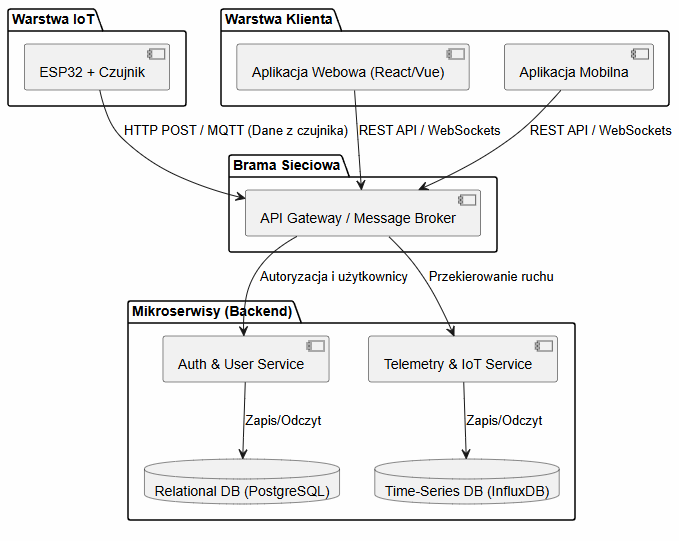
\includegraphics[width=0.7\textwidth]{rysunki/uml.png} 
    \caption{Diagram UML architektury systemu}
    \label{fig:uml} % Klucz dla grafiki PNG
    \sourcefig{opracowanie własne}
\end{figure}

\section{Stos technologiczny}
W celu realizacji projektu wybrano następujące technologie:
\begin{itemize}
    \item Backend: Java, Spring Boot.
    \item Baza danych: MySQL (Docker/XAMPP).
    \item Aplikacja mobilna: Java (Android Studio).
    \item Aplikacja webowa: HTML, CSS, JavaScript.
    \item IoT: C++, ESP32 (Arduino).
\end{itemize}

\section{Wykorzystany sprzęt}
Do realizacji projektu wykorzystano następujące urządzenia:
\begin{itemize}
    \item Mikrokontroler ESP32 Wroom.
    \item Czujnik temperatury DHT11.
    \item Komputer stacjonarny (serwer).
    \item Smartfon z systemem Android (klient).\\
\end{itemize}

W celu realizacji projektu został wypożyczony zestaw ESP32 Wroom wraz z czujnikiem DHT11, który umożliwił odczyt danych pomiarowych i ich bezprzewodową transmisję do serwera. Jak pokazano na rysunku \ref{fig:esp32}, urządzenie zostało odpowiednio podłączone według schematu połączeń przedstawionego na rysunku \ref{fig:esp32_schemat} i przygotowane do pracy w ramach systemu monitorowania temperatury.
\begin{figure}[H]
    \centering
    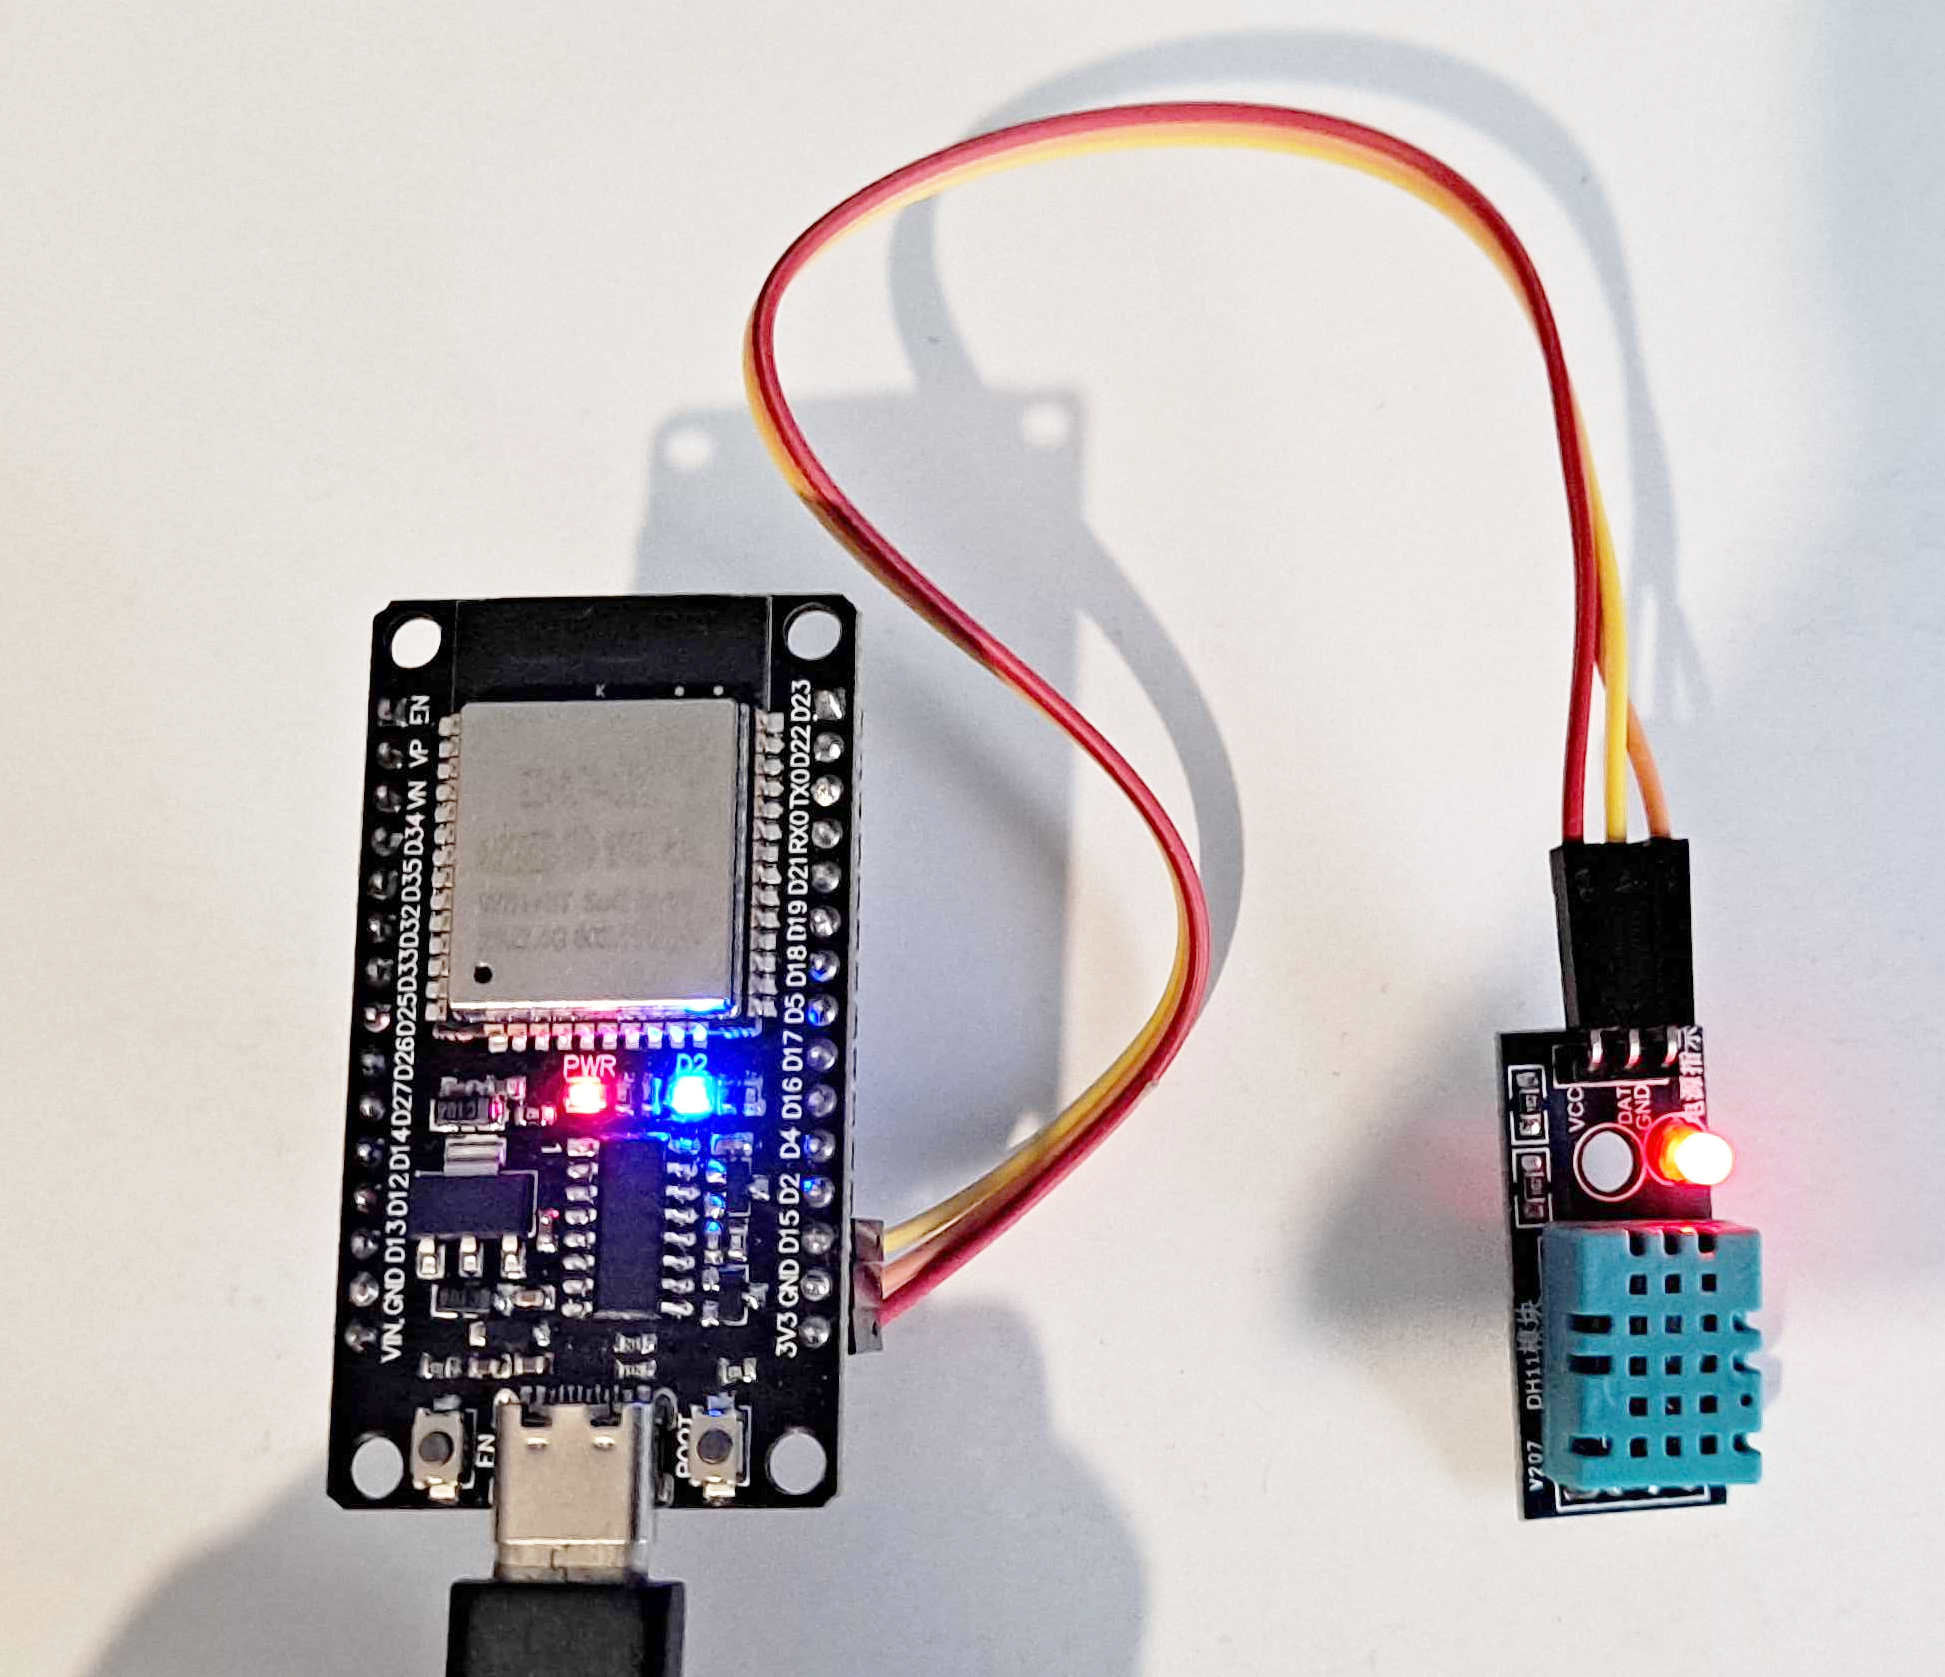
\includegraphics[width=0.7\textwidth]{rysunki/esp32.png} 
    \caption{ESP32 Wroom z czujnikiem DHT11}
    \label{fig:esp32} % Klucz dla grafiki PNG
    \sourcefig{opracowanie własne}
\end{figure}

Schemat połączeń elektrycznych pomiędzy mikrokontrolerem ESP32 a czujnikiem temperatury i wilgotności DHT11 przedstawiono na rysunku \ref{fig:esp32_schemat}. Linia danych (DAT) czujnika została podłączona do pinu GPIO15 mikrokontrolera, natomiast zasilanie zrealizowano poprzez wyprowadzenia 3V3 oraz GND.
\begin{figure}[H]
    \centering
    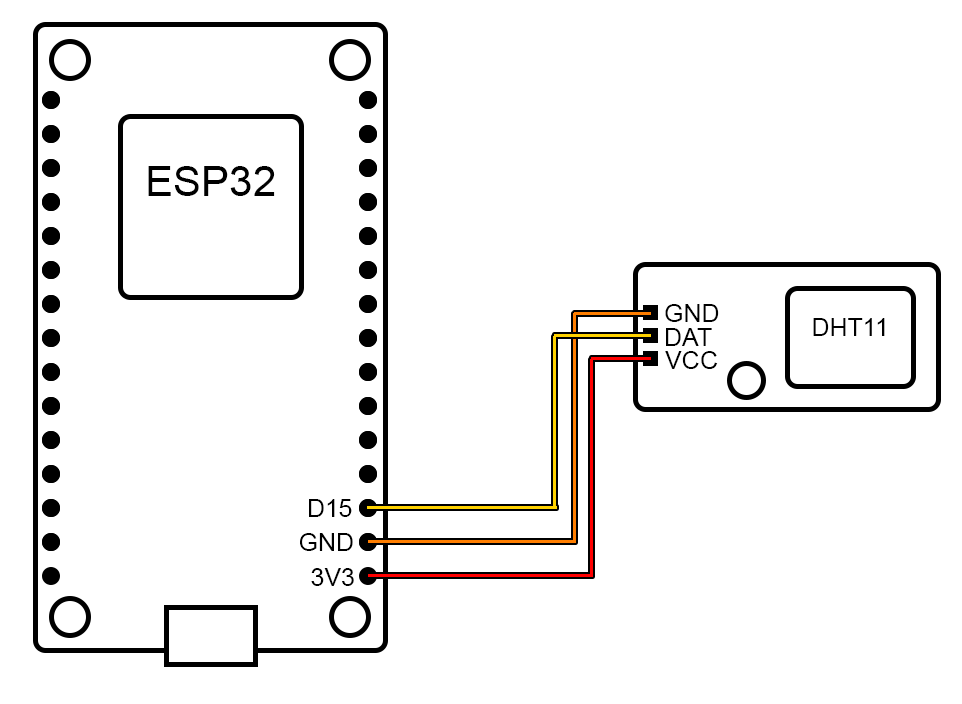
\includegraphics[width=0.5\textwidth]{rysunki/schemat.png} 
    \caption{Schemat połączeń ESP32 z czujnikiem DHT11}
    \label{fig:esp32_schemat} % Klucz dla grafiki PNG
    \sourcefig{opracowanie własne}
\end{figure}

\section{Schemat płytki PCB}
Płytka PCB została zaprojektowana w programie EasyEDA, co pozwoliło na precyzyjne rozmieszczenie elementów oraz przygotowanie modelu do ewentualnej produkcji. Schemat płytki przedstawiono na rysunku \ref{fig:pcb}, gdzie widoczne są połączenia między mikrokontrolerem ESP32 a czujnikiem DHT11.
\begin{figure}[H]
    \centering
    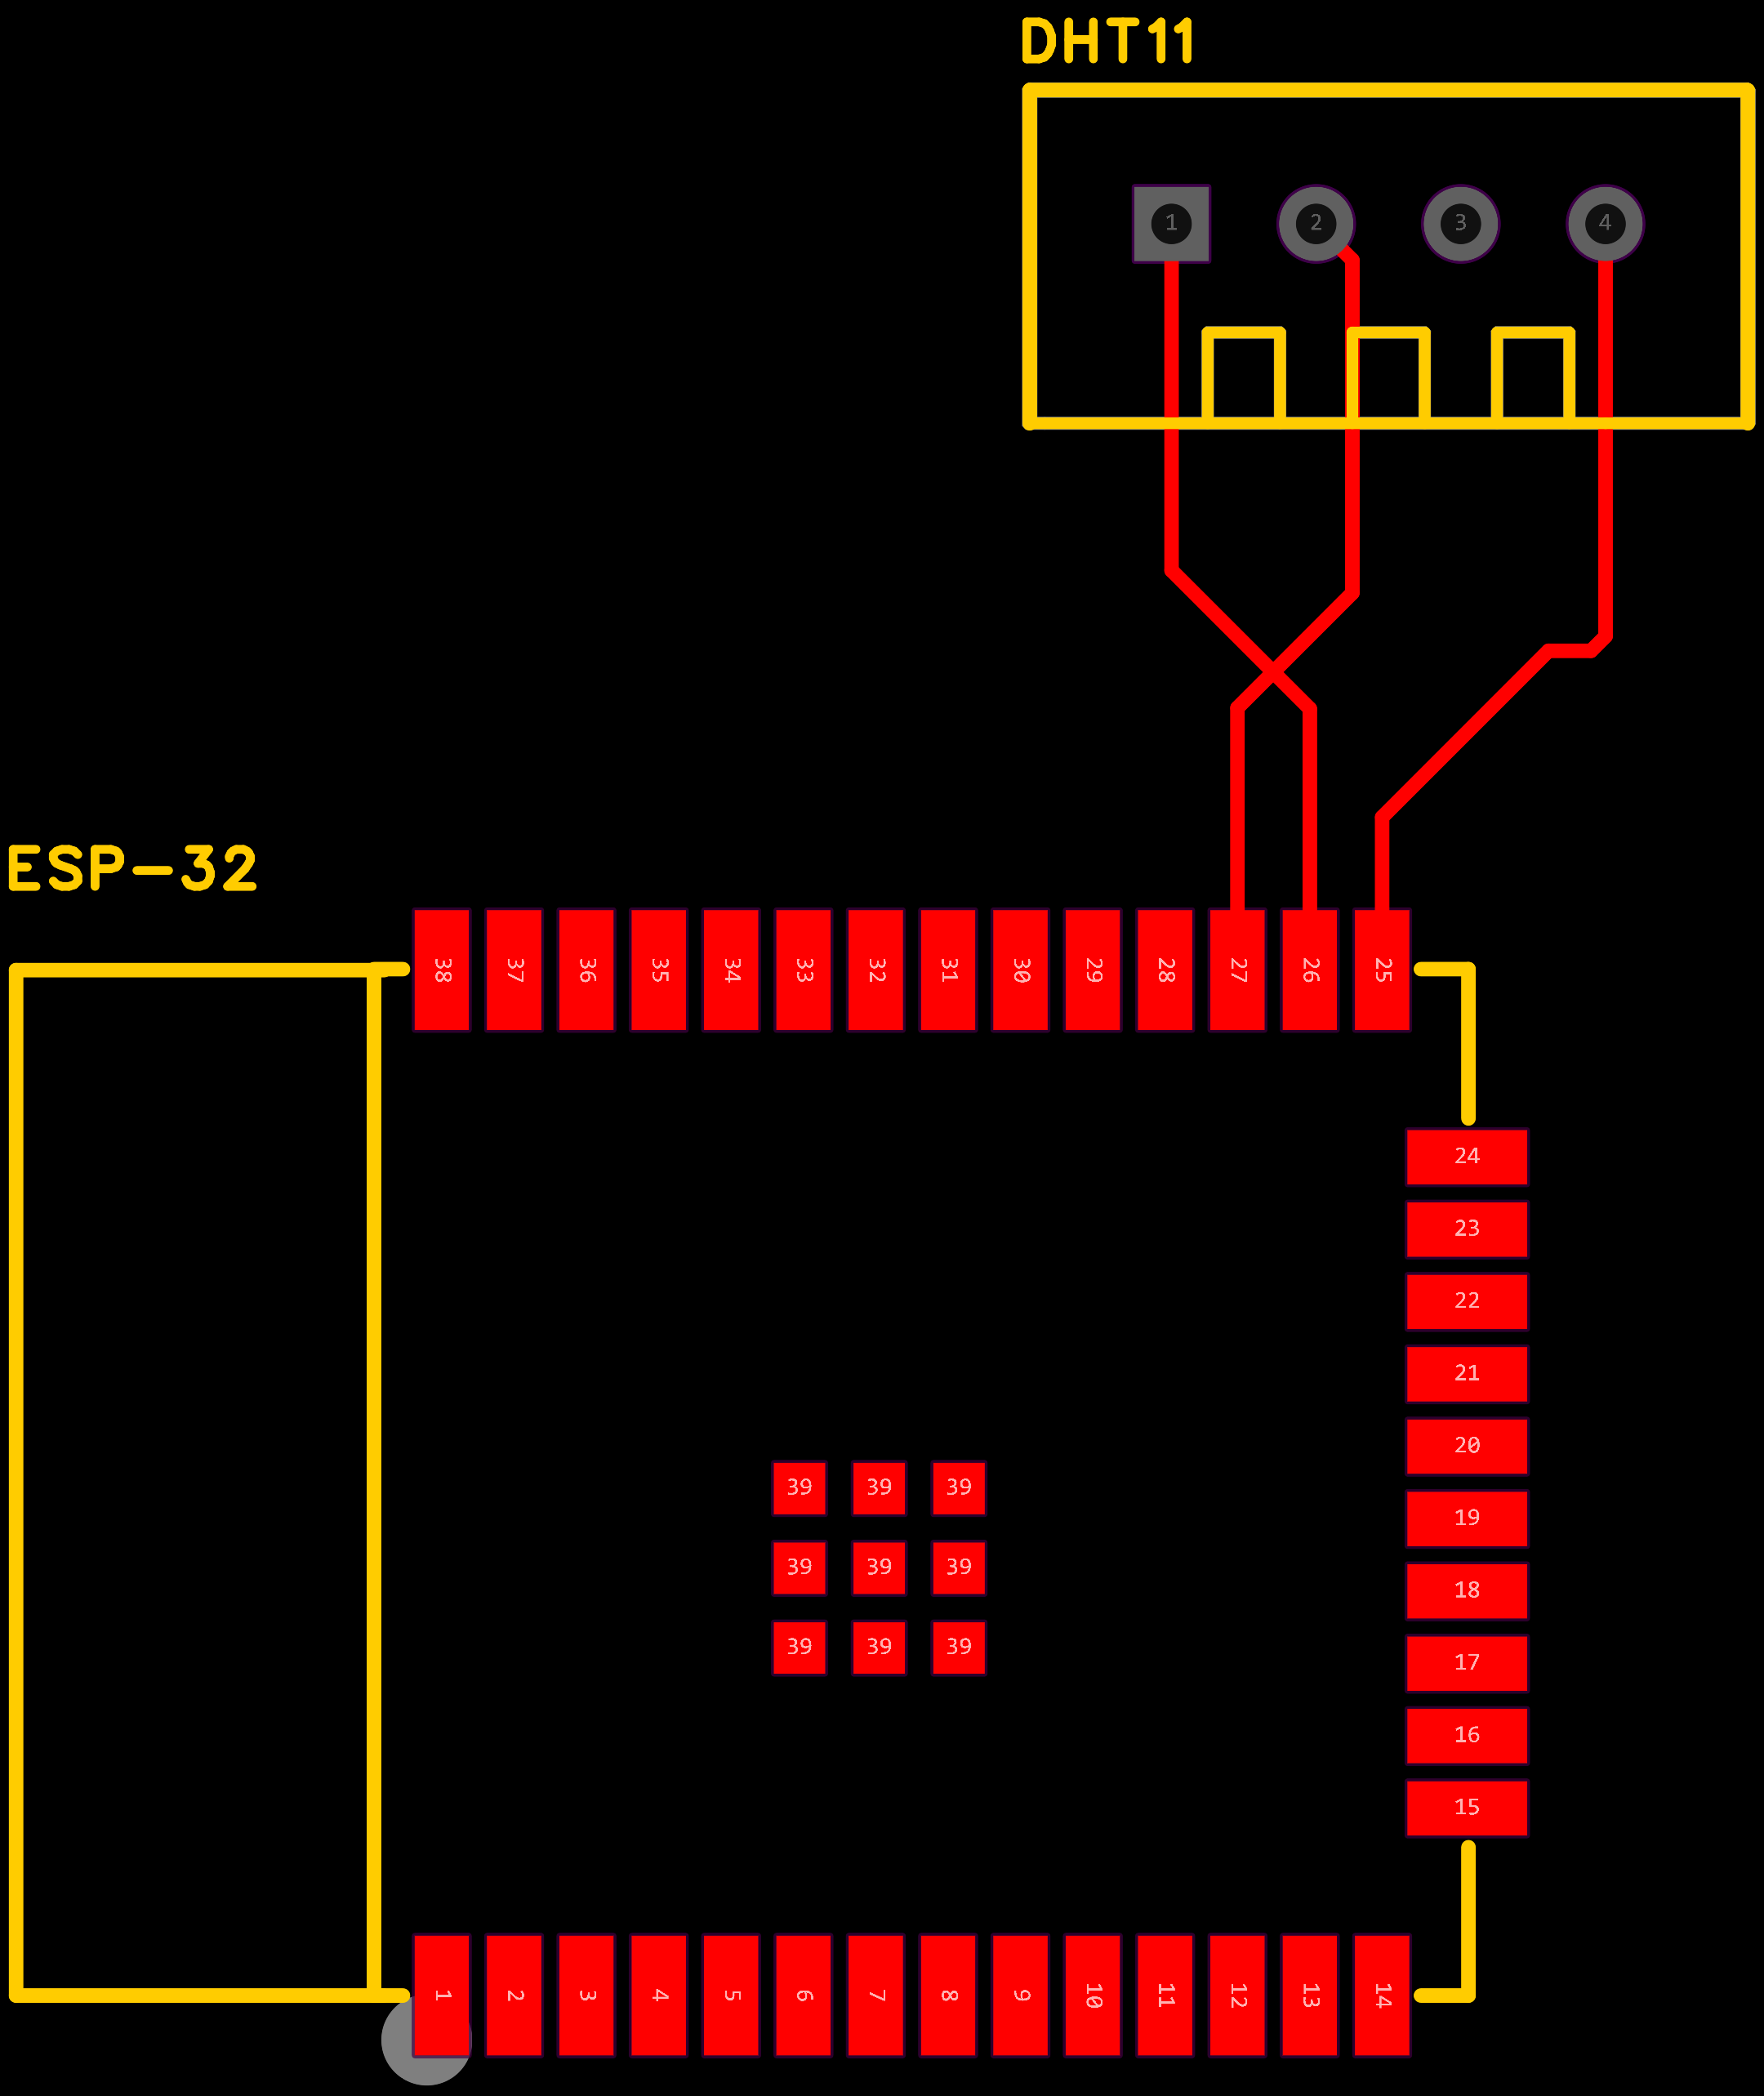
\includegraphics[width=0.4\textwidth]{rysunki/pcb2d.png} 
    \caption{Schemat płytki PCB}
    \label{fig:pcb} % Klucz dla grafiki PNG
    \sourcefig{opracowanie własne (EasyEDA)}
\end{figure}

Sporządzona została też wizualizacja 3D płytki PCB, która umożliwia lepsze zrozumienie rozmieszczenia komponentów oraz ich wzajemnych połączeń. Jak pokazano na rysunku \ref{fig:pcb3d}, model 3D przedstawia szczegółowy układ elementów na płytce, co jest istotne dla dalszych etapów produkcji i montażu.
\begin{figure}[H]
    \centering
    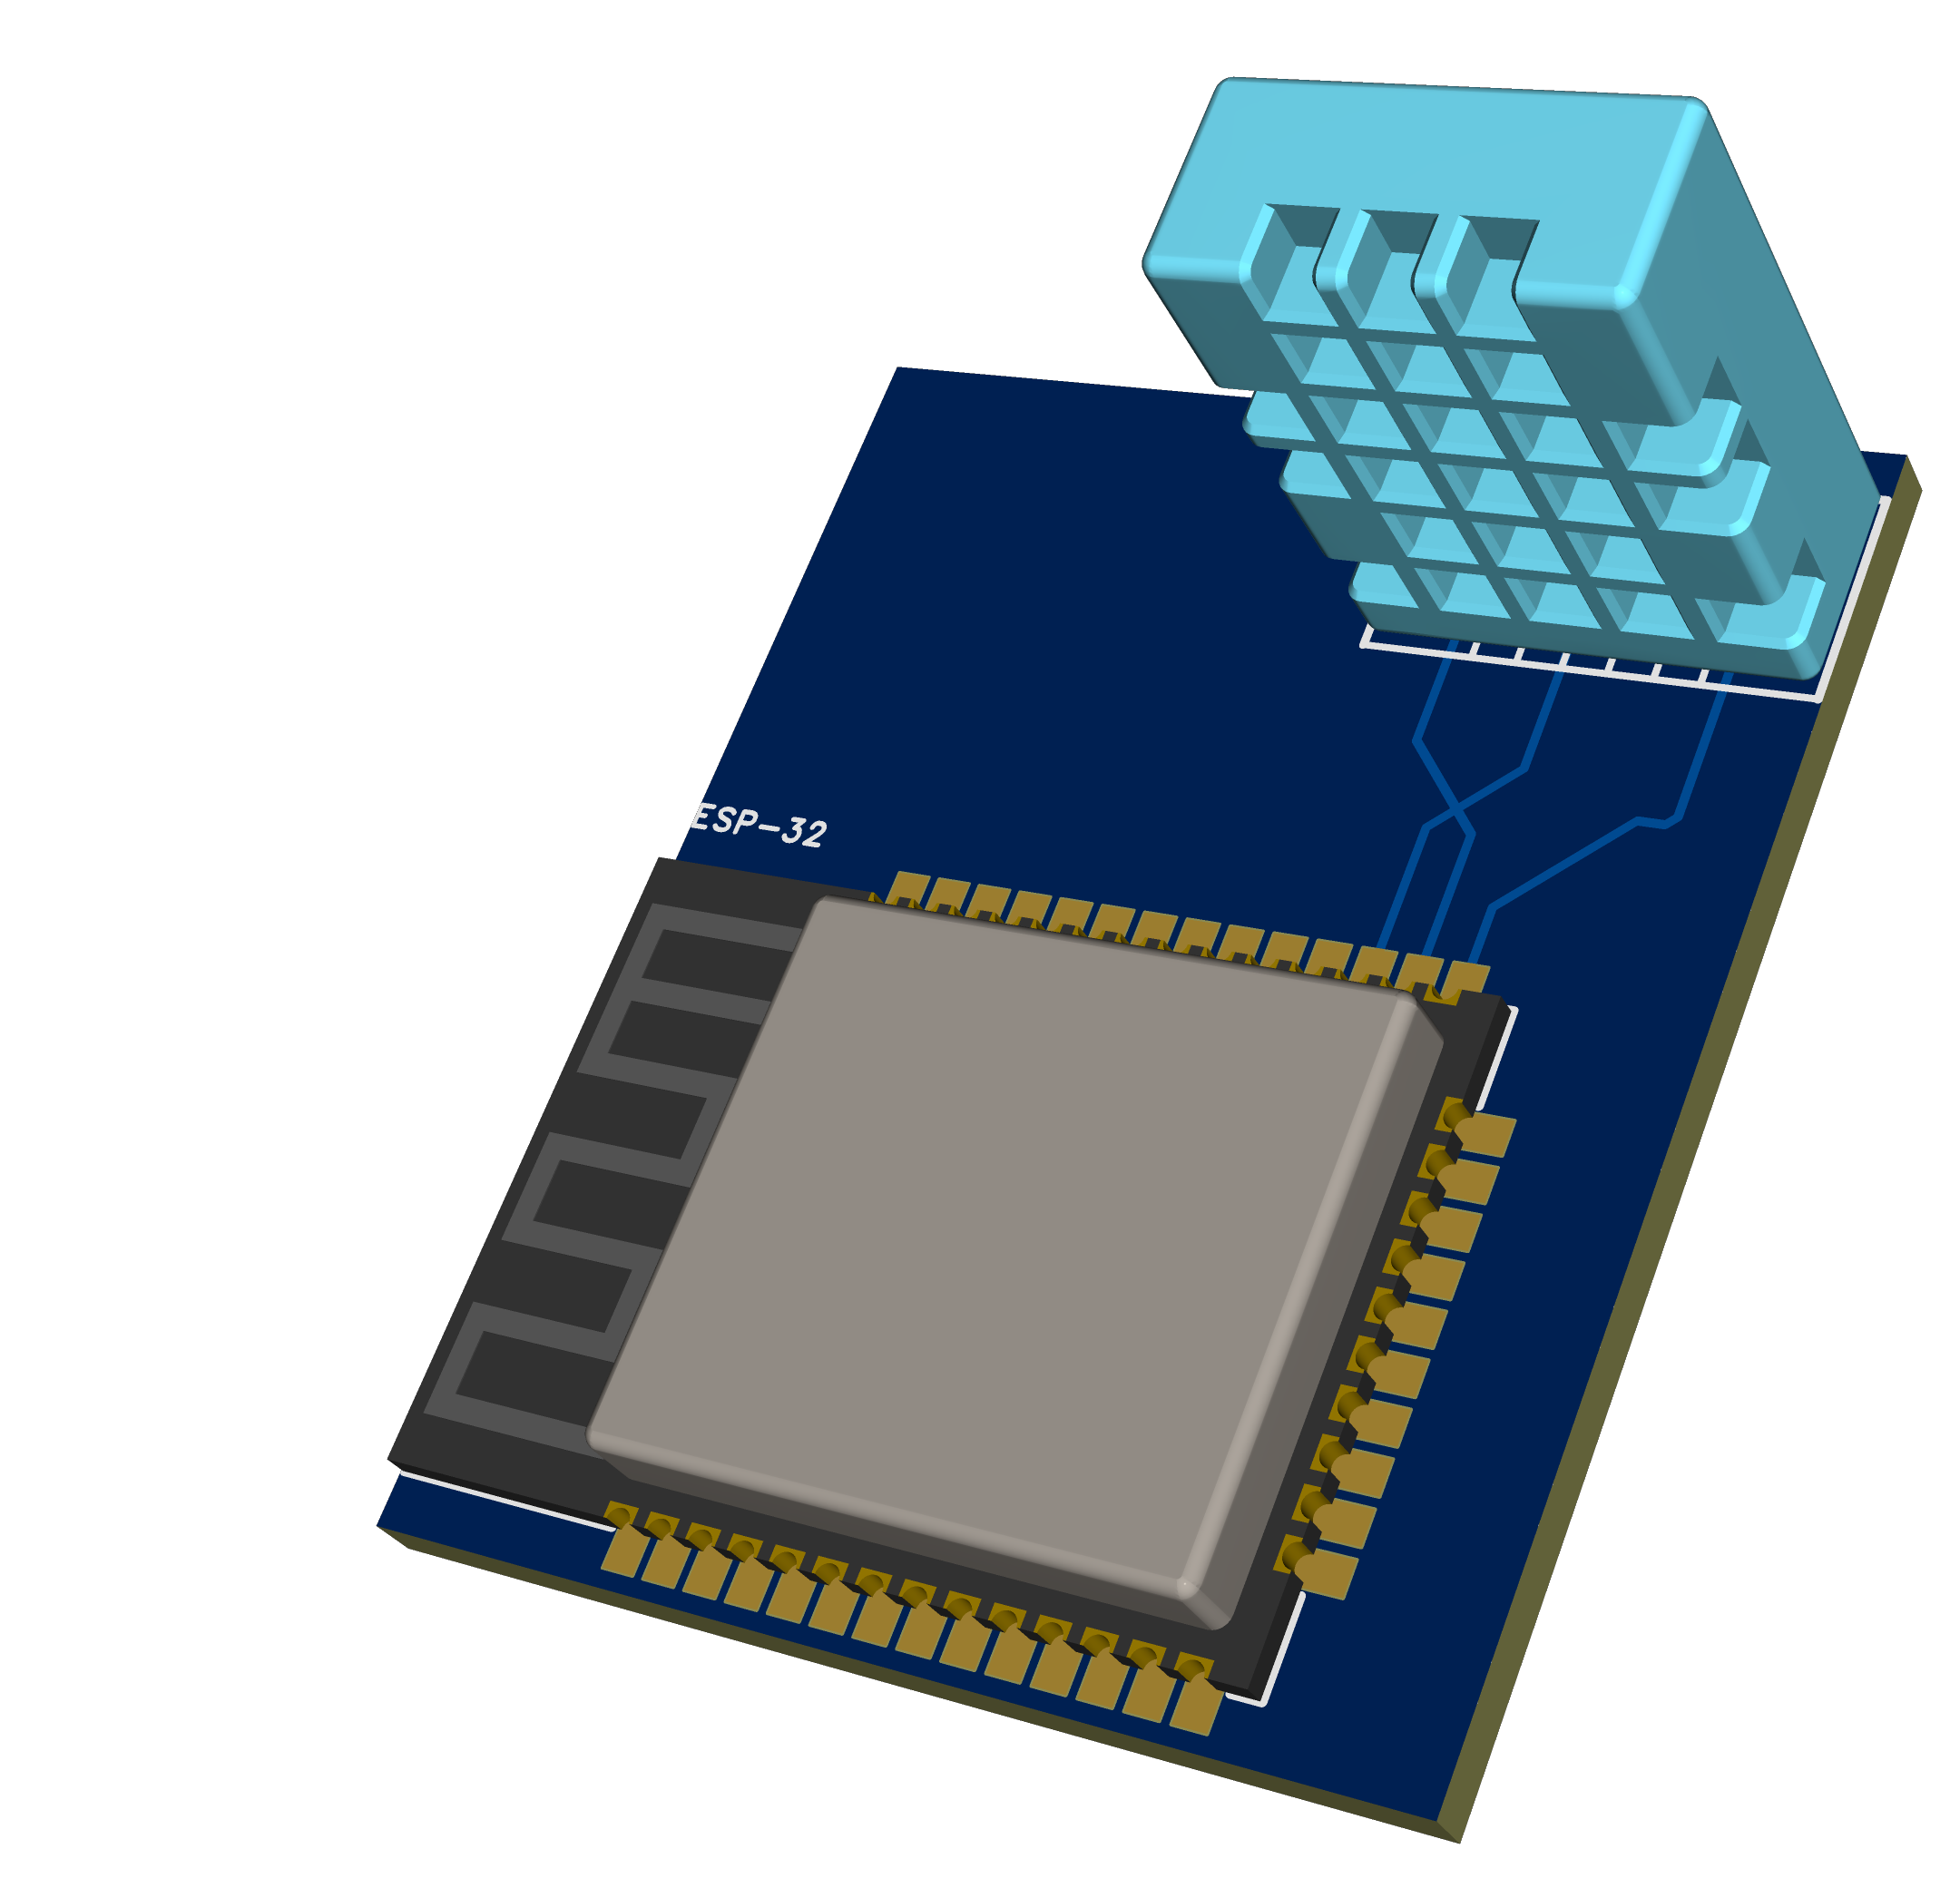
\includegraphics[width=1\textwidth]{rysunki/pcb3d.png} 
    \caption{Wizualizacja przestrzenna płytki PCB}
    \label{fig:pcb3d} % Klucz dla grafiki PNG
    \sourcefig{opracowanie własne (EasyEDA)}
\end{figure}